\begin{figure}
    \begin{subfigure}{.5\textwidth}
    \includegraphics[width=\linewidth,height=0.7\textwidth]{graphics/mutdistribution_.png}
    \caption{Skin-Melanoma}
    \label{fig:density_skin}
    \end{subfigure}
    ~
    \begin{subfigure}{.5\textwidth}
    
    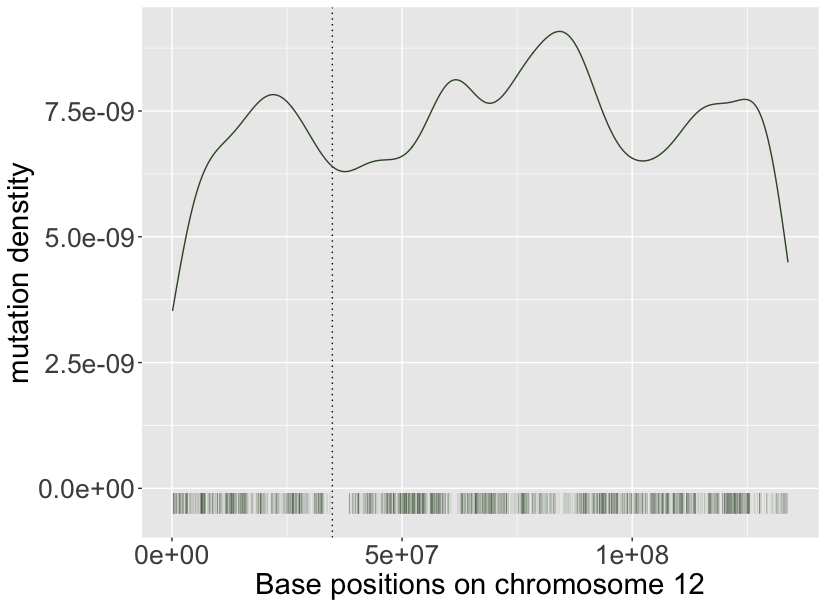
\includegraphics[width=\linewidth,height=0.7\textwidth]{graphics/mutdistribution_Kidney-RCC.png}
    \caption{Kidney-RCC}
    \label{fig:density_kidney}
    \end{subfigure} \\
    \vspace{0.5cm}
    
    \begin{subfigure}{.5\textwidth}
    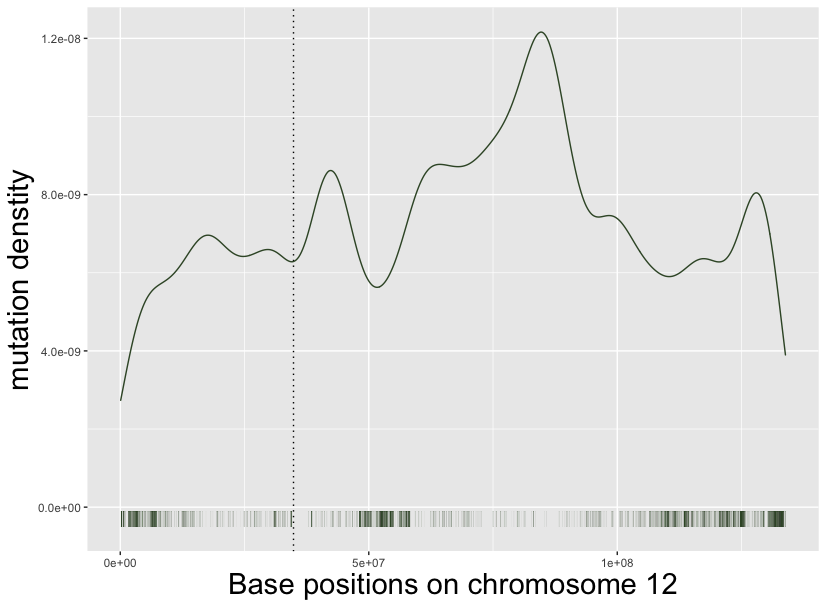
\includegraphics[width=\linewidth,height=0.7\textwidth]{graphics/mutdistribution_Liver-HCC.png}
    \caption{Liver-HCC}
    \label{fig:density_liver}
    \end{subfigure}
    ~
    \begin{subfigure}{.5\textwidth}
    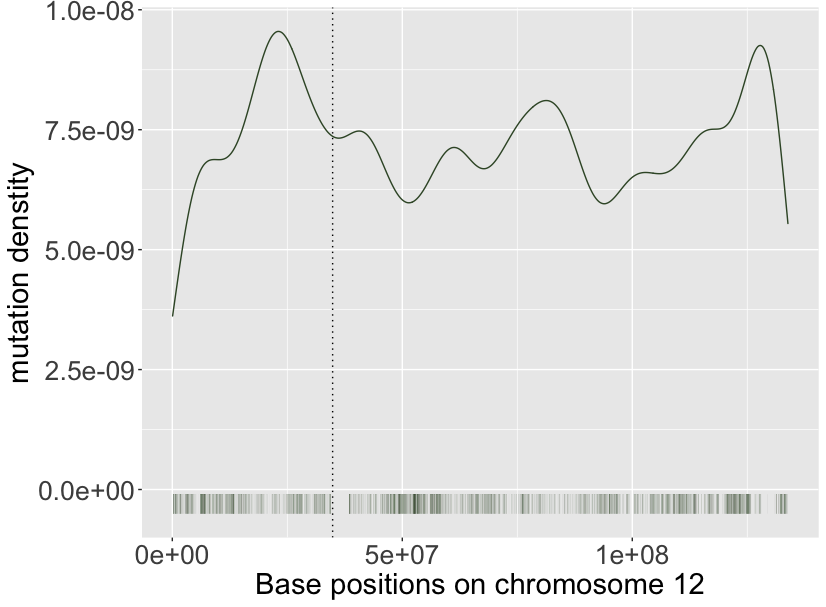
\includegraphics[width=\linewidth,height=0.7\textwidth]{graphics/mutdistribution_Panc-AdenoCA.png}
    \caption{Panc-AdenoCA}
    \label{fig:density_panc_adenoca}
    \end{subfigure} \\
    
    \caption{\textbf{Mutations tend to be found in closed chromatin regions.} Different cancers differ in the distribution of mutations across the genome. Here chromosome 12 is shown. (a) Skin-Melanoma (b) Kidney-RCC (c) Liver-HCC (d) Panc-AdenoCA. The green bar below the x-axis indicates hypersensitivity regions, the gap indicates closed chromatin regions. The vertical dotted line indicates the position of the centromere.}
    \label{fig:mutation_density}
\end{figure}